
%\documentclass[xcolor=pdftex,dvipsnames,table]{beamer}
\documentclass[xcolor=pdftex,dvipsnames,table]{beamer}

\usetheme{Amsterdam}

\usefonttheme[onlymath]{serif}
\setbeamertemplate{navigation symbols}{}
\setbeamertemplate{footline}[frame number]

%\usepackage{paralist}
%\usepackage{enumerate}

\usepackage{colortbl}
\usepackage{lmodern}
\usepackage{comment}
\usepackage{natbib}
\usepackage{graphicx}
\usepackage{pbox}
\usepackage{pifont}
\usepackage{alltt}
\usepackage{verbatim}
\usepackage{multirow}
\usepackage{xspace}
\usepackage{cases}
\usepackage{geometry}
\usepackage{verbatim}
\usepackage{tikz}
\usepackage{pgf}
\usetikzlibrary{arrows,automata,positioning}
%\usepackage[absolute,overlay]{textpos}
\usepackage[normalem]{ulem}
\usepackage{tikz-qtree}
\usepackage{pbox}
\usepackage{amsopn}
%\usepackage{enumitem}
%\usepackage{ragged2e}
%\usepackage{pifont}

%\usepackage[all]{xy}

\usepackage{latexsym}
\usepackage{amsmath}
\usepackage{amssymb}
\usepackage{xfrac}
\usepackage{algorithmicx}
\usepackage{algpseudocode}

\usepackage{notation}
\usepackage{variables}
\usepackage{drawing}
%\usepackage{xparse}
%\usepackage{tikz}
%\usetikzlibrary{calc}
\usepackage{changepage}

\newcounter{savedenum}
\newcommand*{\saveenum}{\setcounter{savedenum}{\theenumi}}
\newcommand*{\resume}{\setcounter{enumi}{\thesavedenum}}



% declares a document
\begin{document}



	%\title{Employee's social media use}
	%\title{Social media use by employees}
	\title{Latent-variable CRF for SMT}
	%\subtitle{for unsupervised language learning}

	\author{Wilker Aziz}
	\institute[UvA]{
		%\inst{1}
		Universiteit van Amsterdam\\
		\texttt{w.aziz@uva.nl}
	}

	\date{\today}
	
	% Title page
	{\setbeamertemplate{footline}{}
	\begin{frame}[plain]
		\titlepage
	\end{frame}
	}

	%\frame{
	\frametitle{Decoding for SMT}
	
	\pause 
	We will be reasoning \\ \pause
	\begin{center}
		making decisions
	\end{center}
	
	\pause
	
	~ about solutions \\ \pause
	\begin{center}
		structures (translations)
	\end{center}
	
	\pause
	
	~ under a statistical model \\ \pause
	\begin{center}
		a function / a partial ordering
	\end{center}
	
	
}

\frame{
	\frametitle{Keywords}
	
	We need to better characterise 
	
	\begin{enumerate}
		\item<2-> space of solutions \\
		\textcolor{blue}{get to know the terrain}
		\item<3-> statistical model \\
		\textcolor{blue}{how to assess the importance of things}
		\item<4-> decision rules \\
		\textcolor{blue}{know what you want}
	\end{enumerate}
	
	
}

\frame{
	\frametitle{Terrain}
	
	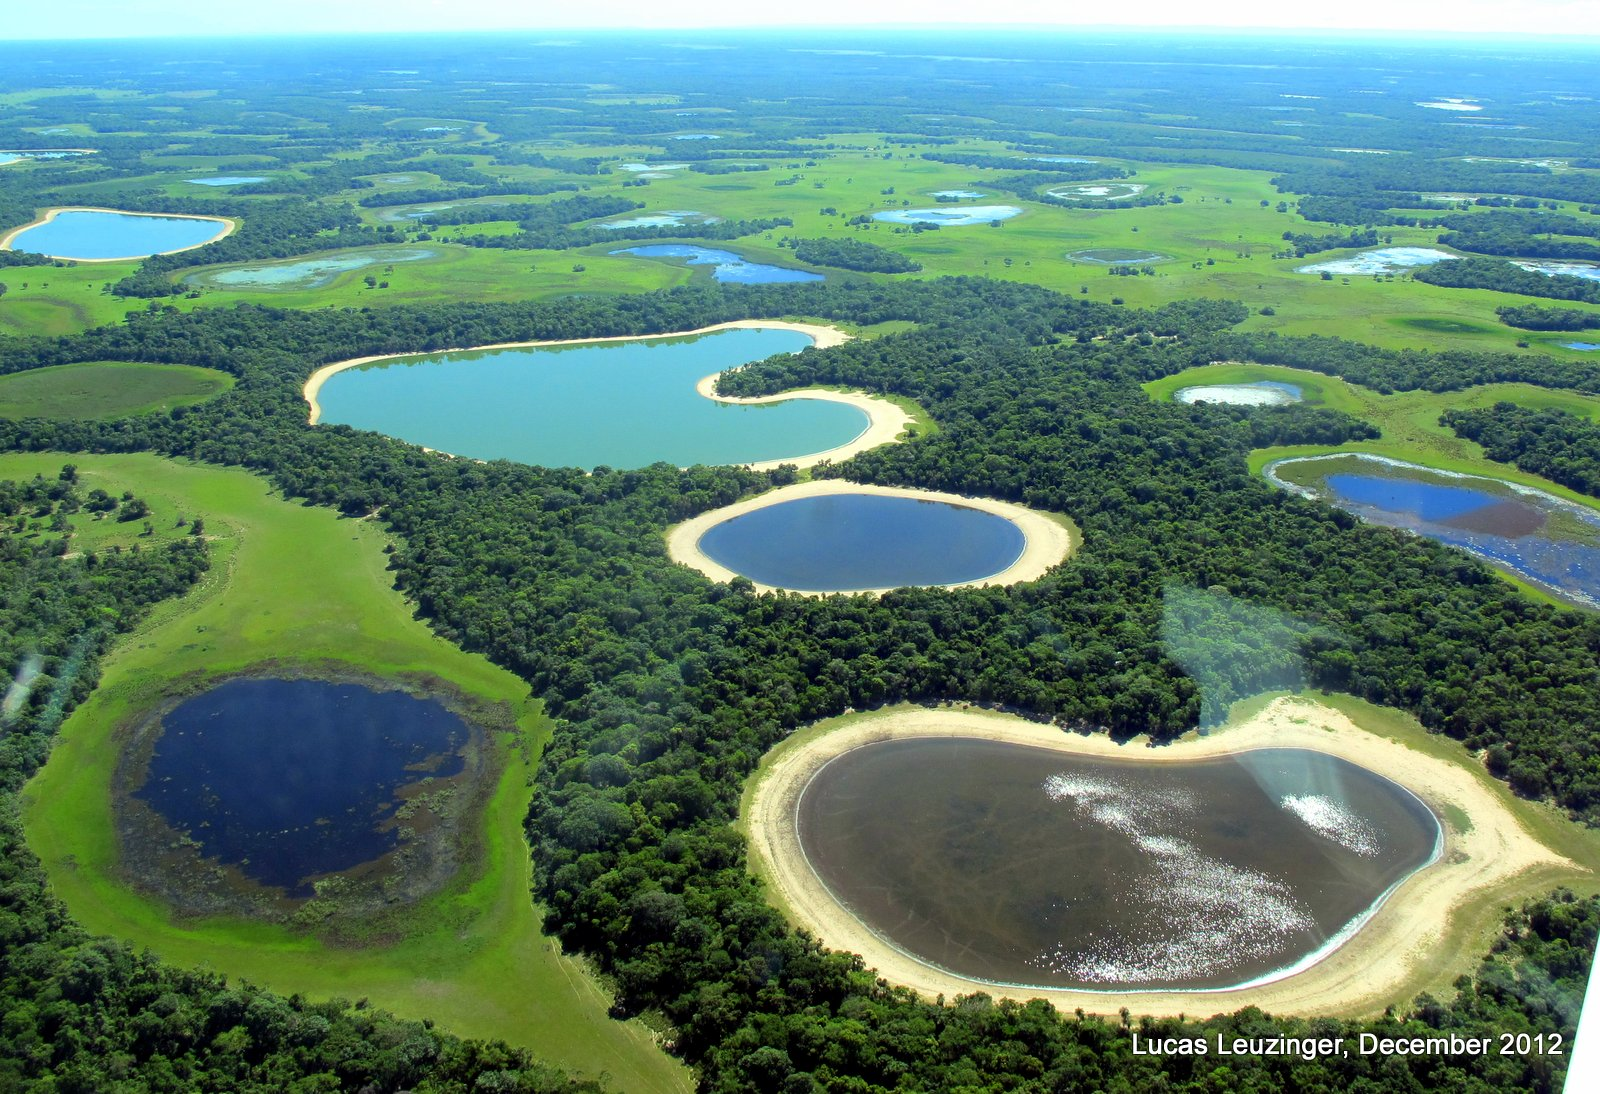
\includegraphics[scale=0.4]{img/pantanal} \pause
	
	not everywhere is a good place to stand
}

\frame{
	\frametitle{The importance (or cost) of things}
	
		
		\only<1>{
	
		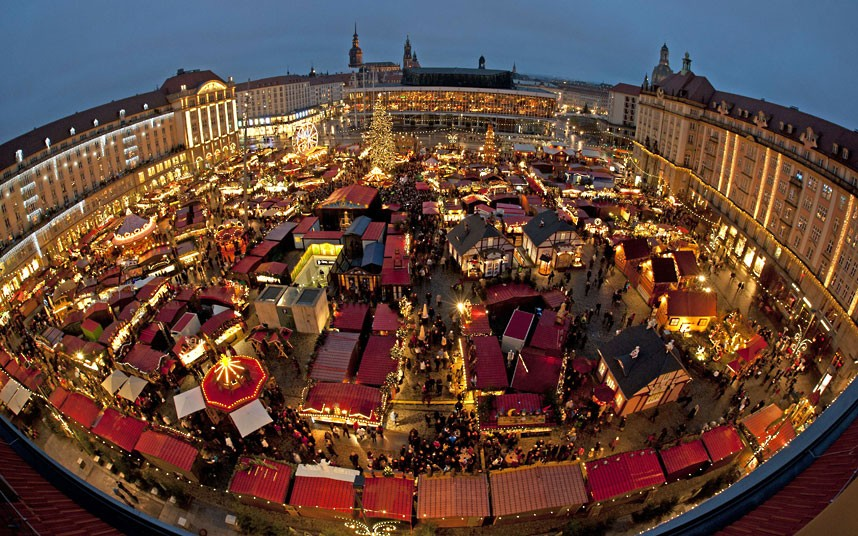
\includegraphics[scale=0.3]{img/demarket} 
		
		German xmas market
		
		}

		\only<2>{
		
		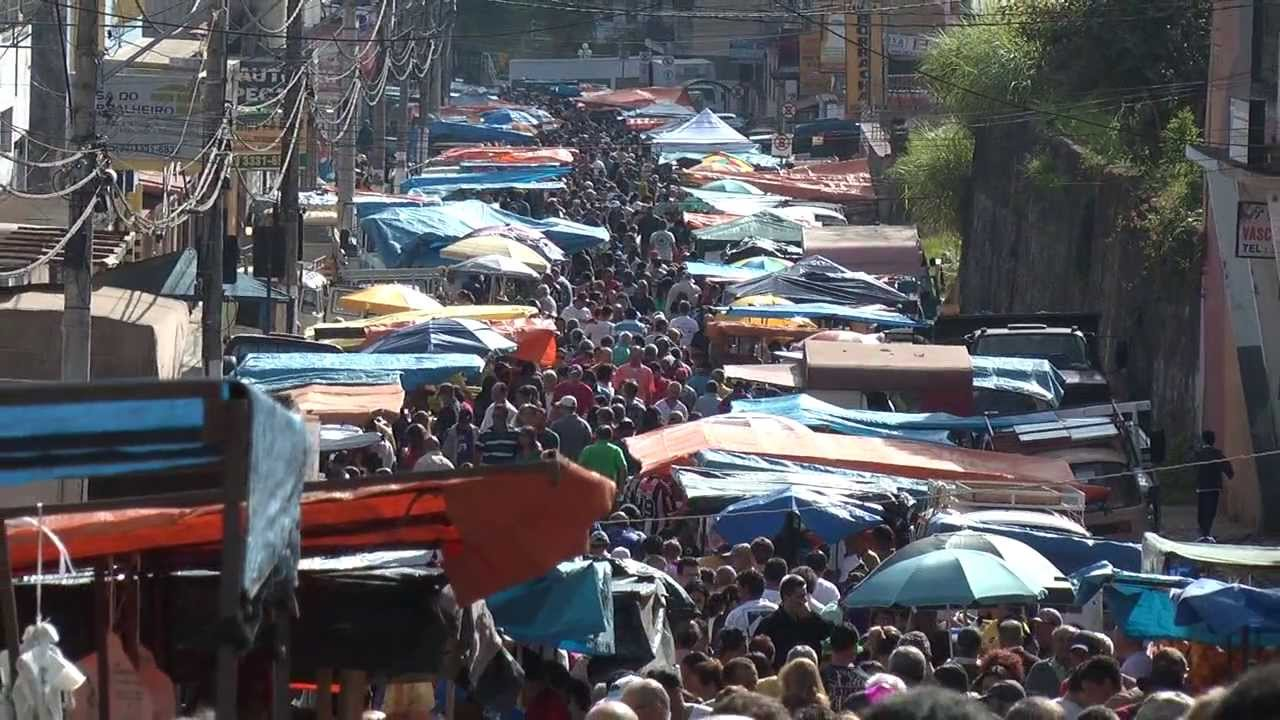
\includegraphics[scale=0.2]{img/brmarket}
		
		Brazilian street market
		
		}
		\only<3-6>{
		
			German xmas market
			\begin{columns}
				\begin{column}{0.4\textwidth}
					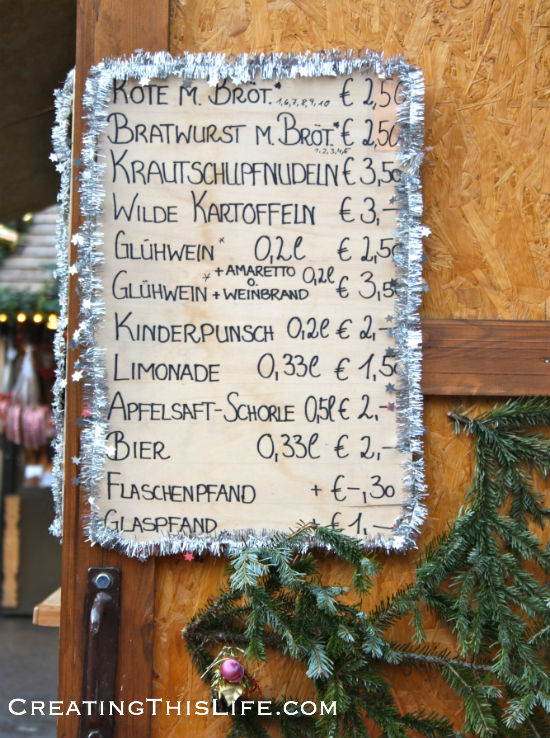
\includegraphics[scale=0.2]{img/demenu}
				\end{column}
				\begin{column}{0.45\textwidth}
					Price of product depends on
					\begin{itemize}
						\item<4-> the product
						\item<5-> brand
						\item<6-> quality of service
					\end{itemize}
				\end{column}
			\end{columns}
		}

		\only<7->{
		
			Brazilian street market
			\begin{columns}
				\begin{column}{0.4\textwidth}
					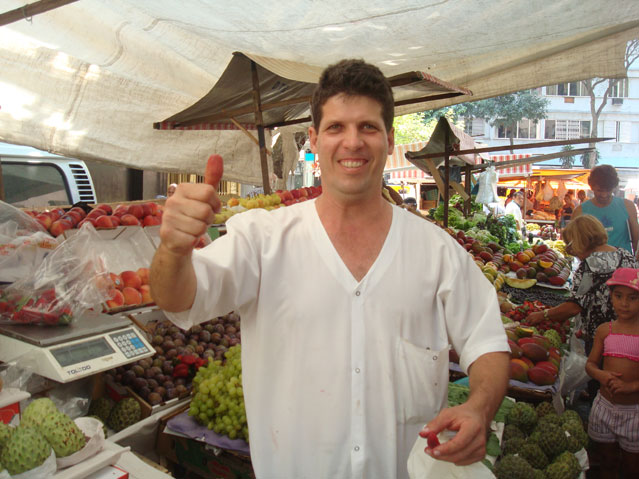
\includegraphics[scale=0.2]{img/feirante}
				\end{column}
				\begin{column}{0.45\textwidth}
					Price of product depends on
					\begin{itemize}
						\item the product
						\item brand
						\item quality of service
						\item<8-> seller's mood
						\item<9-> your look
						\item<10-> products you acquired from other stalls
						\item<11-> from whom you bought those
					\end{itemize}
				\end{column}
			\end{columns}
		}

}

\frame{
	\frametitle{Know what you want}
	
	\only<1>{
		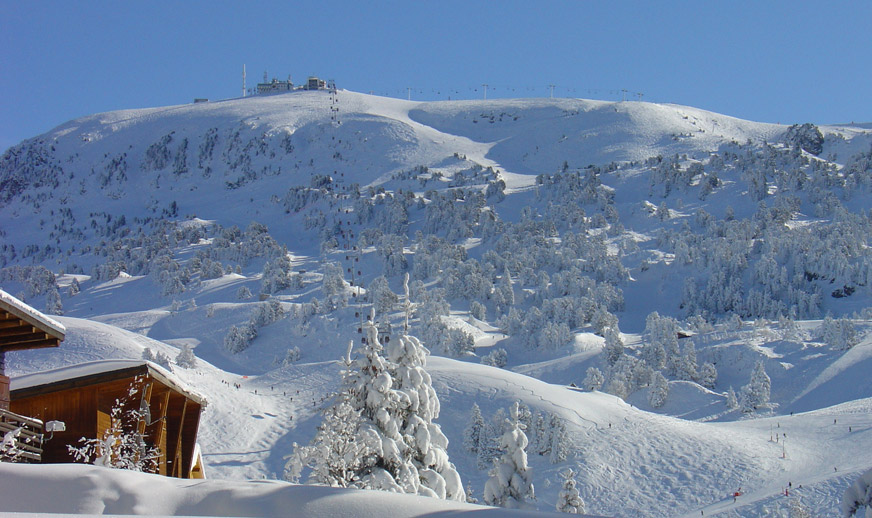
\includegraphics[scale=0.3]{img/station}
		
		what do you think when you see this picture?
	}
	\only<2>{
		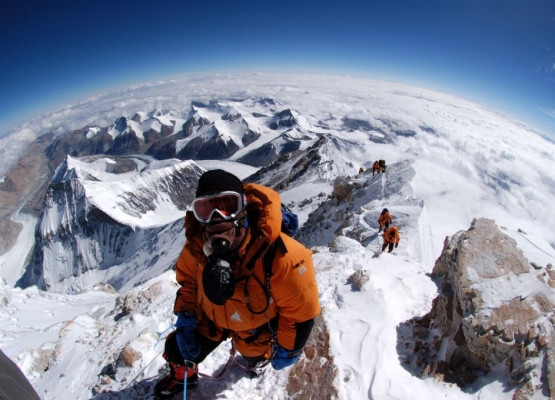
\includegraphics[scale=0.4]{img/top}
		
		make a selfie (and lose a couple of fingers in the process)?
	}
	\only<3>{
		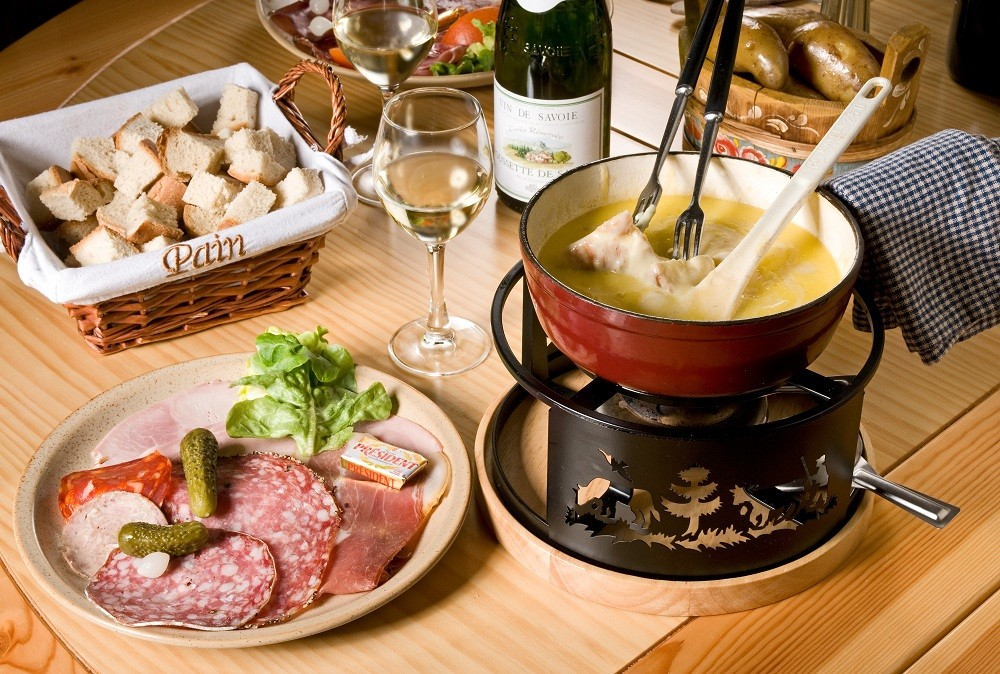
\includegraphics[scale=0.25]{img/dinner}
		
		French goodies in a cozy chalet?
	}
}




	% trick to start counting from the table of contents
	\setcounter{framenumber}{0}


	% SLIDES
	
\section{CRF}

\frame{
	\frametitle{Conditional random field}

	\citet{Lafferty+2001:CRF}
	\begin{equation}
		P(y|x,w) = \frac{\exp(w^\top \phi(x, y))}{\sum_{y' \in \mathcal Y(x)} \exp(w^\top \phi(x, y'))}
	\end{equation}
	
	\begin{itemize}
		\item $\phi$ is a feature function mapping $(x, y)$ to $\mathbb R^d$
		\item $w$ is a feature vector in $\mathbb R^d$
		\item $Z(x|w) = \sum_{y \in \mathcal Y(x)} \exp(w^\top \phi(x, y))$ must be finite
	\end{itemize}
}

\frame{
	\frametitle{Flexible (overlapping) features}
	
	Examples
	\begin{center}
		{\bf As}$_1$ menin{\bf as}$_2$ for{\bf am}$_3$ pra$_4$ l\'a$_4$ $\leftrightarrow$ The$_1$ girls$_2$ went$_3$ over$_4$ there$_4$ 
	\end{center}

	~
		
	\begin{center}
	Apague$_1$ a$_2$ luz$_3$ $\leftrightarrow$ Switch$_1$ the$_2$ light$_3$ off$_1$
	\end{center}
	
	~
	
	Hard to account for with directed models \\
	(due to causality assumptions)
}

\frame{
	\frametitle{Global normalisation}
	
	Local models are trained with positive context only
	\begin{itemize}
		\item MLE: maximise the likelihood of observation $(c, o)$ under $P(O|C=c)$ \pause
		\item Label bias \citep{Lafferty+2001:CRF}
	\end{itemize}
	
	\pause
	
	~
	
	What happens when we query the model with predicted contexts? 
	
}

\frame{
	\frametitle{Maximum likelihood estimation}
	
	Likelihood of an observation $(x, y)$
	\begin{align}
		\mathcal L(w|x, y) &= \log P(y|x,w) \\
		&= w^\top \phi(x, y) - \log Z(x|w)
	\end{align}
	
	\pause
	
	Gradient-based optimisation
	\begin{align}
		\nabla_w \mathcal L(w|x, y) &= \phi(x, y) - \mathbb E_{P(Y|X=x, w)}[\phi(X, Y)]
	\end{align}
	
	\pause
	Expected features should match the features of the observation
}

\section{CRF with latent variables}

\frame{
	\frametitle{LV-CRF}

	Model
	\begin{equation}
		P(y, d|x) = \frac{\exp(w^\top \phi(x, y, d))}{\sum_{y' \in \mathcal Y(x)} \sum_{d' \in \mathcal D(x, y')} \exp(w^\top \phi(x, y', d'))}
	\end{equation}
	
	
	\begin{itemize}
		\item $d$ is latent
		\item $Z(x, y|w) = \sum_{d \in \mathcal D(x, y)} \exp(w^\top \phi(x, y, d))$ must be finite
	\end{itemize}
}

\frame{
	\frametitle{MLE for LV-CRF}
	
	Likelihood of an observation $(x, y)$
	\begin{align}
		\mathcal L(w|x, y) &= \log P(y|x,w) \\
		&= \log \sum_{d \in \mathcal D(x, y)} P(y, d|x, w)
	\end{align}
	
	~\pause
	
	Gradient-based optimisation \citep{Mann+2007:EG}
	\begin{align}
		\nabla_w \mathcal L(w|x, y) &= \mathbb E_{P(D|X=x, Y=y, w)}[\phi(X, Y, D)] \\
		&\quad - \mathbb E_{P(Y, D|X=x, w)}[\phi(X, Y, D)]
	\end{align}
	
	\pause
	Expected features should match the features of the expected observation

}

\frame{
	\frametitle{Note on training}
	
	Undirected models are considerably harder to learn
	\begin{itemize}
		\item expensive global normalisation
		\item complex joint distributions
	\end{itemize}
	
	\pause
	
	Particularly hard with latent variables
	\begin{itemize}
		\item Alignment: \citet{Dyer+2011:UWA} 
		\item SMT: \citet{Blunsom+2008:LVMSMT} and \citet{Blunsom+2008:PIMT} \pause
		\item Approximate techniques
		\begin{itemize}
			\item Contrastive divergence \citep{Hinton:2002:PoE}
			\item Contrastive estimation \citep{Smith+2005:CE} 
			\item Piecewise training \citep{Sutton+2005:PTU}
		\end{itemize}
	\end{itemize}
}

\section{LV-CRF for SMT}

\frame{
	\frametitle{SMT with CRFs}
	
	\citet{Blunsom+2008:LVMSMT}
	\begin{itemize}
		\item $d$ is a derivation complying with a \emph{hiero} grammar
		\item $\phi$ featurises steps in a synchronous derivation
		\begin{small}
		$$P(y,d|x) = \frac{\displaystyle\exp\left(\displaystyle \sum_{r_{s,t} \in d} w^\top \phi(r_{s,t}|x, y, d)\right)}{\displaystyle\sum_{d' \in \mathcal D(x)} \exp\left(\displaystyle\sum_{r_{s,t} \in d} w^\top \phi(r_{s,t}|x, y', d')\right)}$$
		\end{small}
		\item $\mathcal D(x)$ is the space of derivations over target strings aligned to the source string $x$
		\item in the denominator $y'$ is defined implicitly as $\text{yield}(d')$
		\item $r_{s,t}$ is a synchronous rule decorated with a source span $s$ and a target span $t$	
	\end{itemize}
	
}

\frame{
	\frametitle{ITG with CRFs}

	In Project 2, you will use an ITG
	\begin{tabular}{l l l}
		$S$ & $\rightarrow$ & $X$ \\
		$X$ & $\rightarrow$ & $X ~ X$ \\
		$X$ & $\rightarrow$ & $x/y$  for all $x \in \Sigma$ and $y \in \Delta$\\
		$X$ & $\rightarrow$ & $\epsilon/y$ for all $y \in \Delta$\\
		$X$ & $\rightarrow$ & $x/\epsilon$ for all $x \in \Sigma$\\
	\end{tabular}

}

\frame{
	\frametitle{Global normalisation}
	
	ITGs are capable of unbounded insertion \hfill (hiero grammars are not!)
	
	~ \pause

	Normaliser may diverge for certain $w \in \mathbb R^d$
	\begin{itemize}
		\item $\mathcal D(x)$ is typically inifinite
		\item $\displaystyle\sum_{d \in \alert{\mathcal D(x)}} \exp\left(\displaystyle\sum_{r_{s,t} \in d} w^\top \phi(r_{s,t}|x, y, d)\right)$
		
	\end{itemize}
	
	~ \pause
	 
	Solution: constrain strings by length
	\begin{itemize}
		\item introduce a constrain $n$ that depends on $x$
		\item make $\mathcal D_n(x)$ such that $|\text{yield}(d)| \le n$ for $d \in \mathcal D_n(x)$
		\item $\displaystyle\sum_{d \in \textcolor{blue}{\mathcal D_n(x)}} \exp\left(\displaystyle\sum_{r_{s,t} \in d} w^\top \phi(r_{s,t}|x, y, d)\right)$
		
	\end{itemize}
}

\frame{
	\frametitle{Learning}
	
	Likelihood of an observation $(x, y, n)$
	\begin{align}
		\mathcal L(w|x, y, n) &= \log P(y|x,n,w) \\
		&= \log \sum_{d \in \mathcal D(x, y)} P(y, d|x, n, w)
	\end{align}
	\hfill note that $\mathcal D(x, y)$ is always finite
	~\pause
	
	Gradient-based optimisation
	\begin{align}
		\nabla_w \mathcal L(w|x, y, n) &= \underbrace{\mathbb E_{P(D|X=x, Y=y, n, w)}[\phi(X, Y, D)]}_{\text{expected features for observation }(x, y)} \\
		&\quad - \underbrace{\mathbb E_{P(Y, D|X=x, n, w)}[\phi(X, Y, D)]}_{\text{expected features for observation }x}
	\end{align}
}

\frame{
	\frametitle{What do we need?}
	
	An ITG parser in order to obtain  \pause
	\begin{enumerate}
		\item $\mathcal D(x)$\\ \pause
		(potentially infinite) set of derivations over target strings that align to the source string $x$ \pause
		\item $\mathcal D_n(x)$\\ \pause
		finite set of derivations over target strings that align to the source string $x$ where the target string is no longer than $n$ words \pause
		\item $\mathcal D(x, y)$\\ \pause
		set of derivations of the string pair $(x, y)$ \pause
		\item expected feature vector of observations $(x, y)$ \pause
		\item expected feature vector of an observation $x$ 
	\end{enumerate}
}

	\section{Decision rules}

\frame{
	\frametitle{Picking one solution}
	
	What do we pick out of the (whole) weighted space of solutions? \\
	
	\begin{itemize}
		\item best translation
		\item ``minimum-loss'' translation
	\end{itemize}
}

\frame{
	\frametitle{Best translation}
	MAP \\
	
	$$\myy\ustar = \argmax_\myy \sum_{\opy[\mdd] = \myy} f(\mdd|\mxx)$$
	
	\pause 
	\begin{itemize}
		\item summing alternative derivations of the same string \\
		NP-complete: related to determinisation \citep{Simaan:1996:complexity} \\ 
	\end{itemize}
	
	\pause
	
	Viterbi (approximation to MAP)\\ 
	
	$$\mdd\ustar = \argmax_\mdd f(\mdd|\mxx)$$
	
	\begin{itemize}
		\item assumes the most likely derivation is enough
	\end{itemize}
}

\frame{
	\frametitle{Minimum Bayes Risk translation}
	
	MBR \\
	\begin{itemize}
		\item<2-> incorporates a loss (or gain) function 
	\end{itemize}
	
	\only<3>{
	$$\myy = \argmin_\myy \angbrack{\loss(\myy, \myy')}_{p(\myy'|\mxx)}$$}
	\only<4>{
	$$\myy = \argmax_\myy \angbrack{\gain(\myy, \myy')}_{p(\myy'|\mxx)}$$}
	\only<5-6>{
	$$\myy = \argmax_\myy \angbrack{\BLEU(\myy, \myy')}_{p(\myy'|\mxx)}$$}
	\only<7-8>{
	$$\myy = \argmax_\myy \sum_{\myy'} \BLEU(\myy, \myy') \alert<8>{p(\myy'|\mxx)}$$}
	\only<9>{
	$$\myy = \argmax_\myy \sum_{\alert<9>{\myy' \sim p(\myy'|\mxx)}} \BLEU(\myy, \myy')$$}
	\only<10->{
	$$\myy = \argmax_\myy \sum_{\myy'} \sum_{\alert<10>{\mdd' \sim p(\mdd'|\mxx)}} \BLEU(\myy, \opy[\mdd'])$$}
	
	\begin{itemize}
		\item<6-> assesses the risk associated with choosing any one translation
		\item<7-> requires the computation of expectations 
		\item<8-> which requires a \alert<8>{probability}
		$$p(\mdd|\mxx) = \frac{f(\mdd|\mxx)}{\sum_{\mdd'} f(\mdd'|\mxx)}$$
		\item<9-> can be estimated by \alert<9>{sampling translations}
		\item<10-> can be estimated from \alert<10>{samples of derivations}
		%\item<11-> \alert{have a look at project 14 ;)}\\
		
	\end{itemize}
}


\section{Decoding algorithms}

\frame{
	\frametitle{DP-based Viterbi}
	
	Explore a truncated version of the full space \pause
	\begin{itemize}
		\item only a budgeted set of outgoing edges form each node \\ \pause
		\begin{itemize}
			\item beam search: exhaustively enumerates outgoing edges, ranks them, prunes all but $k$-best \pause
			\item cube pruning: enumerates $k$ edges in near best-first order \pause
%			\item incremental search: enumerates the $k$-best edges \pause
		\end{itemize}
	\end{itemize}
	
	In order to compare hypotheses more fairly \pause
	\begin{itemize}
		\item future cost estimates \pause
		\item heuristic view of outside weights \pause
		\item cheap dynamic program that estimates the best possible way to complete any translation prefix \pause
	\end{itemize}
	
	\hfill \citep{Koehn+2003:pbsmt} \\
	\hfill \citep{Chiang:2007}
}

\frame{
	\frametitle{DP-based MBR}
	
	Uses derivations in an $n$-best list as samples \pause
	\begin{itemize}
		\item arguably poor proxy to samples \pause
		\item arbitrarily biased (due to pruning) \pause
		\item centred around the Viterbi solution by design (due to beam search)
	\end{itemize}
	\pause
	\hfill \citep{Kumar+2004:MBR}\\
	\hfill \citep{Tromble+2008:LMBR}

}

\frame{
	\frametitle{Sampling}
	
	Gibbs sampling \pause
	\begin{enumerate}
		\item start with a draft translation \pause
		\item resample from posterior (not all simultaneously): \\ segmentation, phrase order, phrase selection \pause
		\item repeat 2 
	\end{enumerate}

	\pause
	Adaptive rejection sampling \pause
	\begin{enumerate}
		\item design a simpler upperbound (e.g. unigram LM) \pause
		\item sample from it \pause
		\item assess or reject at the complex distribution (e.g. $5$-gram LM) \pause
		\item rejected samples motivate refinements of the upperbound \pause
		\item repeat 2-3 until acceptance rate is reasonable (e.g. 5-10\%) 
	\end{enumerate}
	
}

\frame{
	\frametitle{Sampling}

	Disadvantages \pause
	\begin{itemize}
		\item hard to do it without introducing bias \pause
		\item might require large number of samples
	\end{itemize}
	\pause
	
	Advantages \pause
	\begin{enumerate}
		\item broad view of distribution \pause
		\item potential to incorporate arbitrarily complex features \\ 
		(at the sentence level at least) \pause
		\item sometimes unbiased \pause
		\item ideal for MBR and tuning \pause
		\item typically stupid simple to parallelise
	\end{enumerate}
	

}
	
	\frame{
		\frametitle{Roadmap to project 2}
		\begin{enumerate}
			\item understand the parser
			\begin{itemize}
				\item check notes and notebook
			\end{itemize}
			\item implement the constrained forest $\mathcal D_n(x)$
			\item implement feature functions
			\item implement hypergraph algorithms
			\begin{itemize}
				\item topsort, inside, outside, expected features
			\end{itemize}
			\item iterate over mini-batches of data making gradient updates
		\end{enumerate}
	}
	
	\newcounter{finalframe}
	\setcounter{finalframe}{\value{framenumber}}
	
	
	{\setbeamertemplate{footline}{}
    \begin{frame}[plain]{Questions?}
    \end{frame}
  	}
	
	
	%
\frame[plain]{
	\frametitle{Earley intersection}
	
	\begin{footnotesize}
	\begin{align*}
	\textsc{Axioms} & \\
	& \drule{}{\itembrack{S' \ra \bullet S, q, q}}{q \in I} \\
	\textsc{Goal} & \\
	& \itembrack{S' \ra S \bullet, q, r} ~ q \in I \wedge r \in F\\
	\textsc{Scan} & \\
	& \drule{\itembrack{X \ra \alpha \bullet x \beta, q, s}}{\itembrack{X \ra \alpha x \bullet \beta}}{\angbrack{s, x, r} \in E}\\
	\textsc{Predict} & \\
	& \drule{\itembrack{X \ra \alpha \bullet Y \beta, q, r}}{\itembrack{Y \ra \bullet \gamma, r, r}}{Y \ra \gamma \in R} \\
	\textsc{Complete} & \\
	& \drule{\itembrack{X \ra \alpha \bullet Y \beta, q, s}\itembrack{Y \ra \gamma \bullet, s, r}}{\itembrack{X \ra \alpha Y_{s,r} \bullet \beta, q, r}}{X \neq S'} \\
	\textsc{Accept} & \\
	& \drule{\itembrack{S' \ra \bullet S, q, q}\itembrack{S \ra \gamma \bullet, q, r}}{\itembrack{S' \ra  S_{q,r} \bullet, q, r}}{r \in F} 
	\end{align*}
	\end{footnotesize}

	
}




	\frame[allowframebreaks]{ \frametitle{References}
        \bibliographystyle{plainnat}
        \bibliography{../../bib}
	}

	

	% Trick to discount regular frames from the total of backup frames
	\setcounter{framenumber}{\value{finalframe}}
	
	
\end{document}
